%Title: Beamer Presentation Template
%Author: LISA
%Year: 2020

\documentclass[10pt,aspectratio=169]{beamer}
 
%
%Setting file
%

\usepackage[T1]{fontenc}
\usepackage[utf8]{inputenc}

\usepackage[english]{babel}

\usepackage{graphicx}
\graphicspath{{images/}}
\usepackage{float}
\usepackage{tikz}
\usepackage{caption}
\usepackage{subcaption}

\usetheme{default}
\usefonttheme{structurebold}


% ---------------------------------
% color definitions
\usepackage{color}
% \definecolor{LISA_BLUE}{rgb}{0.25,0.33,0.66}
\definecolor{LISA_BLUE}{cmyk}{0.99,0.88,0.29,0.18}

\setbeamercolor{normal text}{fg=LISA_BLUE}
\setbeamercolor{frametitle}{fg=LISA_BLUE}

\newcommand\insertlocation{}  % Empty by default.
\newcommand\location[1]{\renewcommand\insertlocation{#1}}

\newcommand\insertperiod{}  % Empty by default.
\newcommand\period[1]{\renewcommand\insertperiod{#1}}



\setbeamertemplate{itemize items}[circle]
\setbeamercolor{title}{fg=white}



%-----------------------------------------Title page settings-----------------------------------------%
\title{Proton-induced fusion-evaporation reactions for actinide production at IGISOL}
\subtitle{}
\author{\small A. Raggio$^{1}$, I. Moore$^{1}$, I. Pohjalainen$^{2}$, \\ E. Rey-Herme$^{3}$, J. Saren$^{1}$, M. Vandebrouck$^{3}$}
\institute{$^{1}$ Jyv\"{a}skyl\"{a} University \\
$^{2}$ GSI Helmholtzzentrum für Schwerionenforschung GmbH\\
$^{3}$ CEA, Universite Paris-Saclay}
\period{}
\date{May 26, 2021}
\location{Event}


%-----------------------------------------Title page settings-----------------------------------------%


\begin{document}

{
  \usebackgroundtemplate{
\includegraphics[width=\paperwidth]{Title.pdf}}
	\begin{frame}[noframenumbering, plain]
		\titlepage
	\end{frame}
}

\begin{frame}{Content}
	\begin{textblock*}{0.5\paperwidth}(0.03\paperwidth,0.2\paperheight)
		\vspace{0.2\textheight}
		\begin{itemize}
			\item Physics Case
			\item Actinide Quest at IGISOL
			\item Proton-induced Fusion-evaporation\\ with actinide targets
		\end{itemize}
	\end{textblock*}
	\begin{textblock*}{0.5\paperwidth}(0.47\paperwidth,0.2\paperheight)
		% \vspace{0.1\textheight}
		\only<1>{\includegraphics[width=\textwidth]{Full_Chart.pdf}}%
		\only<2>{\vspace{0.2\textheight}\includegraphics[width=\textwidth]{IGI-1A-IGISOL_3.pdf}}%
		\only<3>{\vspace{0.2\textheight}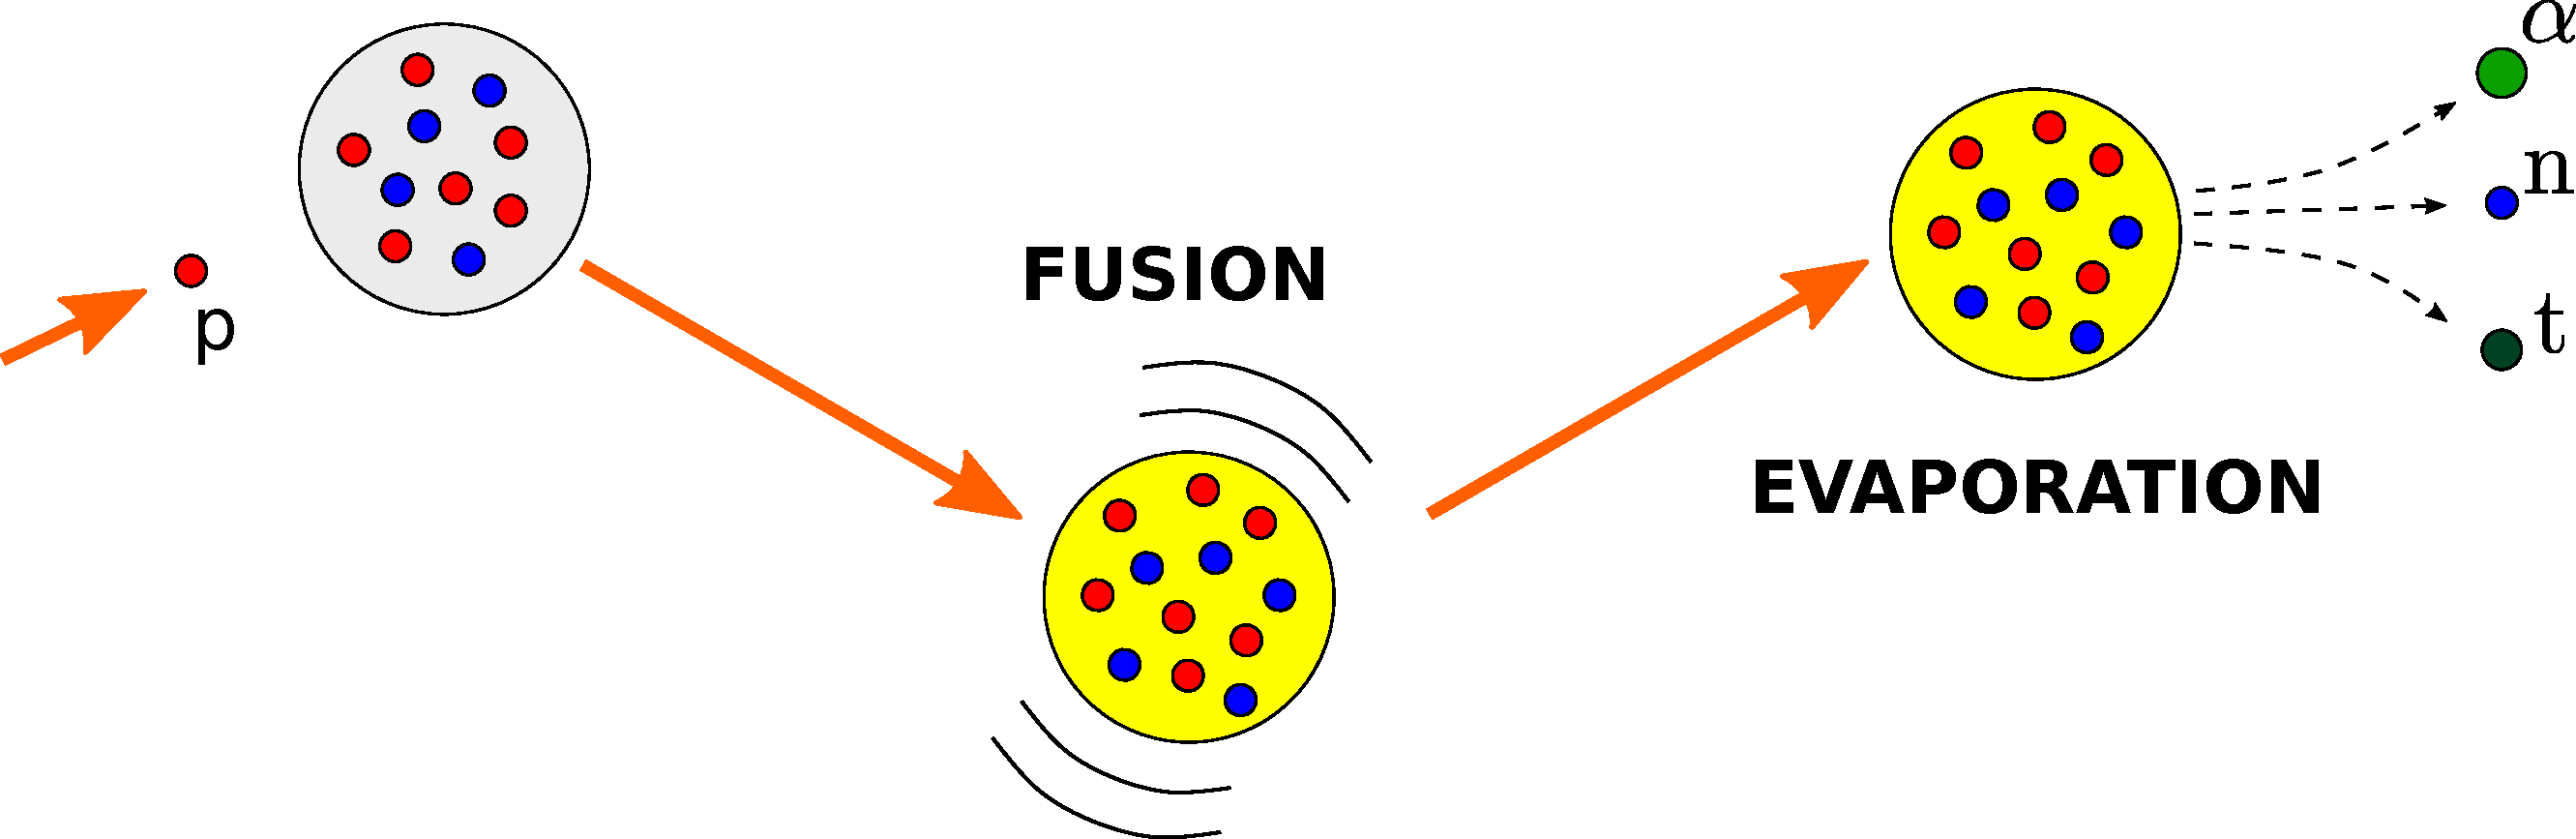
\includegraphics[width=\textwidth]{Reaction.pdf}}%
	\end{textblock*}
\end{frame}

\begin{SectionTitle}
\begin{frame}
	\centering
	\begin{textblock*}{0.5\paperwidth}(0.25\paperwidth,0.2\paperheight)
		\centering
		\textbf{\LARGE PHYSICS CASE}	
	\end{textblock*}
	\begin{textblock*}{0.5\paperwidth}(0.25\paperwidth,0.4\paperheight)
        \includegraphics[width=.8\textwidth]{Full_Chart.pdf}
	\end{textblock*}

\end{frame}
\end{SectionTitle}

\begin{frame}{SLIDE 2}
	An empty fancy slide.
\end{frame}

\end{document}
